% 1982 年全国卷（理科）第 4 题：圆锥及其内接体积最大的圆柱（按源卷布局）。
% 底面半径 R=2.0、高 H=3.4；圆柱底半径 r=0.6、高 h=2.38（源卷约取全高的 0.7）。
% 右侧为 H、h 的尺寸线（均自锥底量起），下方为 2R 的尺寸线。
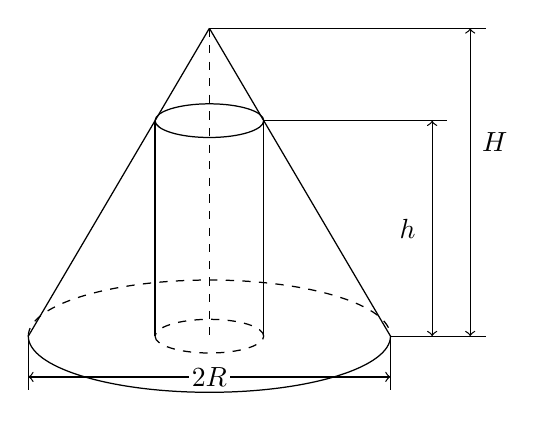
\begin{tikzpicture}[scale=1.15, line width=0.45pt,
  every node/.style={inner sep=1.5pt}]
  % 圆锥底面椭圆（半轴 2.0 与 0.62）：前半（近观者）实线，后半虚线
  \draw (-2.0,0) arc (180:360:2.0 and 0.62);
  \draw[dashed] (-2.0,0) arc (180:0:2.0 and 0.62);
  % 圆锥母线
  \draw (0,3.4) -- (-2.0,0);
  \draw (0,3.4) -- (2.0,0);
  % 圆锥轴（虚线）
  \draw[dashed] (0,3.4) -- (0,0);
  % 圆柱侧面轮廓母线
  \draw (-0.6,0) -- (-0.6,2.38);
  \draw (0.6,0) -- (0.6,2.38);
  % 圆柱上底面（可见，实线椭圆，半轴 0.6 与 0.186）
  \draw (-0.6,2.38) arc (180:360:0.6 and 0.186);
  \draw (0.6,2.38) arc (0:180:0.6 and 0.186);
  % 圆柱下底面（被遮，虚线椭圆）
  \draw[dashed] (-0.6,0) arc (180:360:0.6 and 0.186);
  \draw[dashed] (0.6,0) arc (0:180:0.6 and 0.186);
  % 右侧尺寸线：H 为锥高、h 为圆柱高，均自锥底量起
  \draw (0,3.4) -- (3.05,3.4);
  \draw (2.0,0) -- (3.05,0);
  \draw (0.6,2.38) -- (2.62,2.38);
  \draw[<->] (2.88,0) -- (2.88,3.4);
  \node[right] at (2.96,2.14) {$H$};
  \draw[<->] (2.46,0) -- (2.46,2.38);
  \node[left] at (2.33,1.19) {$h$};
  % 下方尺寸线 2R
  \draw (-2.0,0) -- (-2.0,-0.6);
  \draw (2.0,0) -- (2.0,-0.6);
  \draw[<->] (-2.0,-0.45) -- (2.0,-0.45);
  \node[fill=white, inner sep=1pt] at (0,-0.45) {$2R$};
\end{tikzpicture}
